
\chapter{Oscilador harmónico}

\section{Oscilador armónico}
Analizaremos en detalle la solución a la ecuación de movimiento del oscilador armónico simple que resulta de considerar la fuerza restauradora (en una dimensión)
\begin{align}
  \label{eq:restaur}
  \mathbf{F}=&-kx\hat{\mathbf{i}}\nonumber\\
  F_x=&-kx\,,
\end{align}
en la segunda Ley de Newton (en una dimensión)
\begin{align*}
  F_x=m\ddot{x}\,.
\end{align*}
Usando la ec.~\eqref{eq:restaur} tenemos
\begin{align}
  \label{eq:osci}
  m\ddot{x}+kx=&0\nonumber\\
  \ddot{x}+\omega_0^2 x=&0\nonumber\\
\end{align}donde hemos definido la \emph{frecuencia característica} del oscilador armónico como
\begin{align*}
  \omega_0=\sqrt{\frac{k}{m}}\,.
\end{align*}
Note que la frecuencia característica de un oscilador armónico es por definición positiva y es \emph{característica} de cada oscilador. 

Se propone como solución general a la ecuación diferencial~\eqref{eq:osci}
\begin{align}
  \label{eq:oscisol}
  x=A\cos(\omega_0 t+\phi)\,,
\end{align}
donde $A$ es la amplitud del oscilador y $\phi$ su fase. %(ver figura)
O equivalentemente
\begin{align*}
  x=B\sin(\omega_0 t)+C\cos(\omega_0 t)
\end{align*}
donde
\begin{align}
  B=&-A \sin\phi\,, & C=&A\cos\phi\,.
\end{align}
o en términos de $B$ y $C$
\begin{align}
  \label{eq:BCAphi}
  \tan\phi=&-\frac{B}{C} & A=&\sqrt{B^2+C^2}\,.
\end{align}

$B$ y $C$ ó la amplitud y la fase pueden obtenerse a partir de las condiciones
\begin{align*}
t=&0 & x_0=&x(0)& v_0=&v(0)\,,  
\end{align*}
\begin{align*}
  B=&\frac{v_0}{\omega_0}&  C=&x_0 \nonumber\\
  A=&\sqrt{x_0^2+\frac{v_0^2}{\omega_0^2}}& \tan\phi=&-\frac{v_0}{\omega_0 x_0}\,.
\end{align*}

\subsection{Energía del oscilador armónico}

La fuerza restauradora es una fuerza conservativa que puede obtenerse a partir de la energía potencial
\begin{align*}
  U(x)=\tfrac{1}{2}k x^2\,,
\end{align*}
por lo tanto la energía mecánica del oscilador armónico se conserva. Para encontrar la energía conservada usaremos la solución~\eqref{eq:oscisol} para obtener la energía potencial y cinética en cualquier punto de la oscilación
\begin{align}
\label{eq:osciU}
U(x)=&\tfrac{1}{2}k A^2\cos^2(\omega_0 t+\phi)\,,
\end{align}
\begin{align}
  \label{eq:osciK}
  K(x)=\tfrac{1}{2}k A^2\sin^2(\omega_0 t+\phi)\,.
\end{align}

La energía mecánica es
\begin{align}
  \label{eq:osciE}
  E=&K(x)+U(x)\nonumber\\
  =&\tfrac{1}{2}k A^2\,,
\end{align}
que, en efecto, es constante. 

La Energía mecánica puede relacionarse con cantidades globales asociadas a una oscilación completa. Para ello definimos el promedio de una función sobre un intervalo de tiempo $t_1$ a $t_2$ como
\begin{align*}
  \langle f\rangle=&\frac{1}{(t_2-t_1)}\int_{t_1}^{t_2} f(t) dt\,.
\end{align*}
Si $f(t)=\sin t$, para un período completo del seno entre $0$ y $2\pi$, dado por $T=2\pi$, tenemos:
\begin{align*}
  \langle f\rangle_T=&0
\end{align*}
como puede esperarse de la resta de las dos áreas en el gráfico del seno. %ver figura

Sin embargo, el promedio de $\sin^2t$ es diferente de cero: %ver figura
\begin{align*}
  \langle f^2\rangle_T=&\frac{1}{2}\,,
\end{align*}
de modo que $1/2$ es el valor promedio de $\sin^2 t$. 

Aplicando estos resultados a las funciones de energía potencial y cinética dadas por las ecuaciones \eqref{eq:osciU} y \eqref{eq:osciK}
\begin{align*}
  \langle U\rangle=&\tfrac{1}{4}k A^2\nonumber\\
  \langle K\rangle=&\tfrac{1}{4}k A^2\,,
\end{align*}
y
\begin{align*}
  \langle E\rangle=E\,,
\end{align*}
de modo que la energía mecánica del oscilador armónico coincide con su energía promedio.

El oscilador armónico es un sistema ideal. En la práctica ningún sistema oscila por siempre pues está sometido a fuerzas de amortiguamiento no conservativas debidas a la fricción con el medio que afectan la amplitud (pero no la frecuencia) del oscilador con el tiempo. Una vez el oscilador esta en reposo deber ser forzado, con una fuerza periódica, para regresarlo a su estado de oscilación. Desde el punto de vista práctico es conveniente estudiar las características que debe tener la fuerza periódica para maximizar la amplitud inicial de oscilación y así aumentar el tiempo que dura el sistema oscilando antes de amortiguarse completamente. 

En adelante asumiremos que el oscilador se encuentra inicialmente en reposo en un sistema viscoso y veremos el efecto que tiene una fuerza periódica sobre su movimiento.

\section{Oscilador forzado y amortiguado}
Un oscilador forzado y amortiguado de masa $m$ sufre el efecto combinado de la fuerza restauradora $F_x$ (que depende de la elongación), la fuerza de fricción $f$ (que depende de la rapidez a la que se mueve el oscilador) y una fuerza periódica $\mathcal{F}$ (que depende del tiempo), de modo que está sometido a la fuerza total
\begin{align*}
  F_{\text{total}}=F_x(x)+\mathcal{F}(t)+f(v)\,.
\end{align*}

La fuerza de fricción sobre un objeto moviéndose a través de un fluido líquido o gaseoso  (a bajas velocidades) es usualmente proporcional a la rapidez de su movimiento\footnote{A velocidades altas la fuerza de fricción es proporcional al cuadrado de la rapidez}
\begin{align*}
  f(v)=-b v\,,
\end{align*}
la constante de proporcionalidad depende de la forma y la masa del cuerpo, además de las propiedades del medio a través del cual se mueve el cuerpo. 
El fluido también se denomina medio viscoso. 

A modo de ilustración, si el cuerpo es una placa horizontal sobre la superficie de un líquido que se comporta como un \emph{fluido newtoniano}, como por ejemplo el agua
\begin{align*}
  b=\mu\frac{A}{h}\,,
\end{align*}
donde $\mu$ es el coeficiente de viscosidad, $A$ el área de la placa, y $h$ la altura del fluido.

Sin perdida de generalidad se puede escribir la fuerza periódica aplicada sobre un cuerpo como
\begin{align*}
  \mathcal{F}(t)=\mathcal{F}_0\cos(\omega t)\,,
\end{align*}
donde $\omega$ es la frecuencia de la fuerza aplicada y en general es independiente de la frecuencia propia del oscilador $\omega_0$. 

Con estas consideraciones la fuerza total queda
\begin{align*}
  F_{\text{total}}=-k x -b\dot x+\mathcal{F}_0\cos(\omega t)
\end{align*}
que da lugar a la ecuación de movimiento
\begin{align}
  \label{eq:oscforamo}
  \ddot x+\gamma \dot x+\omega_0^2 x=\frac{\mathcal{F}_0}{m}\cos(\omega t)\,,
\end{align}
donde
\begin{align*}
  \gamma=&\frac{b}{m}&\omega_0^2=&\frac{k}{m}\,,
\end{align*}
donde $\gamma$ y $\omega^2$ tienen unidades de $1/\text{seg}$. En lugar de solucionar directamente esta ecuación diferencial inhomogénea, es decir, que depende explícitamente del tiempo, introducimos una ecuación similar en términos de una variable \emph{imaginaria} $y$
\begin{align*}
    \ddot y+\gamma \dot y+\omega_0^2 y=\frac{\mathcal{F}_0}{m}\sin(\omega t)\,,
\end{align*}
y construimos una ecuación diferencial inhomogénea en términos de la variable compleja $z$
\begin{align}
  \label{eq:oscforamoz}
   \ddot x+i\ddot y+\gamma \dot x+i\gamma \dot y+\omega_0^2 x+i\omega_0^2 y=&
   \frac{\mathcal{F}_0}{m}\left[\cos(\omega t)+i\sin(\omega t)\right]\nonumber\\
    \ddot z+\gamma \dot z+\omega_0^2 z=&\frac{\mathcal{F}_0}{m}e^{i\omega t}\,.
\end{align}
Si logramos solucionar está ecuación, la parte real de dicha solución corresponderá a la solución del oscilador armónico forzado amortiguado~\eqref{eq:oscforamo}.

Proponemos como solución para~\eqref{eq:oscforamoz}
\begin{align}
  \label{eq:propsol}
  z=z_0 e^{i\omega t}
\end{align}

de donde %detalles
\begin{align}
  \label{eq:soluz}
  (-\omega^2+i\omega\gamma+\omega_0^2)z_0=&\frac{\mathcal{F}_0}{m}\nonumber\\
  (\omega_0^2+i\omega\gamma-\omega^2)z_0=&\frac{\mathcal{F}_0}{m}\,,
\end{align}
De esta ecuación podemos despejar $z_0$, para luego obtener su magnitud y fase
\begin{align*}
  z_0=&\frac{\mathcal{F}_0}{m}\frac{1}{\omega_0^2+i\omega\gamma-\omega^2}\nonumber\\
  =&\frac{\mathcal{F}_0}{m}\frac{1}{(\omega_0^2-\omega^2)+i\omega\gamma}
\frac{(\omega_0^2-\omega^2)-i\omega\gamma}{(\omega_0^2-\omega^2)-i\omega\gamma}\nonumber\\
  =&\frac{\mathcal{F}_0}{m}\frac{(\omega_0^2-\omega^2)-i\omega\gamma}{(\omega_0^2-\omega^2)^2+\omega^2\gamma^2}\nonumber\\
  =&\frac{\mathcal{F}_0}{m}\frac{(\omega_0^2-\omega^2)}{(\omega_0^2-\omega^2)^2+\omega^2\gamma^2}-
i\frac{\mathcal{F}_0}{m}\frac{\omega\gamma}{(\omega_0^2-\omega^2)^2+\omega^2\gamma^2}\nonumber\\
=&x_0+iy_0\,,
\end{align*}
donde
\begin{align*}
  x_0=&\frac{\mathcal{F}_0}{m}\frac{(\omega_0^2-\omega^2)}{(\omega_0^2-\omega^2)^2+\omega^2\gamma^2}\nonumber\\
  y_0=&-\frac{\mathcal{F}_0}{m}\frac{\omega\gamma}{(\omega_0^2-\omega^2)^2+\omega^2\gamma^2}\,.
\end{align*}
Podemos escribir $z_0$ en coordenadas polares encontrando su magnitud y fase
\begin{align}
  \label{eq:rphiz0}
  \phi=&\tan^{-1}\left(\frac{\omega\gamma}{\omega^2-\omega_0^2}\right)\nonumber\\
  |z_0|^2=&x_0^2+y_0^2\nonumber\\
  =&\left(\frac{\mathcal{F}_0}{m}\right)^2\frac{(\omega_0^2-\omega^2)^2+\omega^2\gamma^2}{%
    \left[(\omega_0^2-\omega^2)^2+\omega^2\gamma^2\right]^2}\nonumber\\
  =&\left(\frac{\mathcal{F}_0}{m}\right)^2\frac{1}{%
    (\omega_0^2-\omega^2)^2+\omega^2\gamma^2}\,.
\end{align}
Expandiendo la solución en \eqref{eq:propsol}
\begin{align}
  z=&z_0 e^{i\omega t}\nonumber\\
  =&|z_0|e^{i\phi}e^{i\omega t}\nonumber\\
  =&|z_0|\exp[i(\omega t +\phi)]\nonumber\\
  =&|z_0|\cos(\omega t+\phi)+i|z_0|\sin(\omega t+\phi)\nonumber\\
  =&x(t)+iy(t)\,,
\end{align}

Usando las ecs.~\eqref{eq:rphiz0}, llegamos finalmente a %detalles
\begin{align}
  \label{eq:soluforzamo}
  x(t)=A(\omega)\cos(\omega t+\phi)\,,
\end{align}
donde
\begin{align}
  \label{eq:aomega}
  A(\omega)=|z_0|=&\frac{\mathcal{F}_0}{m}\frac{1}{\left[\left(\omega_0^2-\omega^2\right)^2+\gamma^2\omega^2\right]^{1/2}}\nonumber\\
  \phi=&\tan^{-1}\left(\frac{\omega\gamma}{\omega^2-\omega_0^2}\right).
\end{align}
La solución queda completamente especificada sin tener que usar las condiciones iniciales. %discusión al respecto


\subsection{Oscilador forzado}
En ausencia de fricción con el medio viscoso, $\gamma=0$ y la ec.~\eqref{eq:aomega} se reduce a
\begin{align*}
  A(\omega)=&\frac{\mathcal{F}_0}{m}\frac{1}{\omega_0^2-\omega^2}\nonumber\\
  \phi=&\tan^{-1}0=0\,,
\end{align*}
de modo que la solución \eqref{eq:soluforzamo} queda 
\begin{align*}
  x(t)=\frac{\mathcal{F}_0}{m}\frac{1}{\omega_0^2-\omega^2}\cos(\omega t)
\end{align*}
La amplitud de oscilación $A(\omega)$ es máxima, de hecho $\pm$infinita, cuando $\omega\to \omega_0$ a izquierda y derecha, como se ilustra en la figura~\ref{fig:resonance}
\begin{frame}
  \begin{figure}
    \centering
    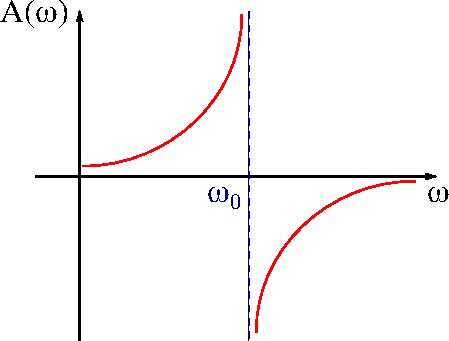
\includegraphics[scale=0.9]{resonance}
    \caption{Resonancia}
    \label{fig:resonance}
  \end{figure}
\end{frame}


Cuando la frecuencia de forzado $\omega$ es igual a $\omega_0$, se dice que se está operando a la \emph{frecuencia de resonancia}. Operar en resonancia permite obtener amplitudes grandes para fuerzas impulsoras pequeñas, como ocurre por ejemplo en los tubos de órganos, o en el sintonizador de una radio. Un caso extremo es la bah{ia de Fundy en Canada, donde el período del oleaje para ir de un lado al otro de la bahía y el tiempo entre dos mareas altas (12.4 horas) es similar, lo que produce olas de mas de $\SI{10}{\meter}$.  En otras aplicaciones es necesario reducir la respuesta a una resonancia, como en la suspensión de un automóvil donde una fuerza viscosa es utilizada para disipar energía. 

\example{}
Explique para un punto $A(\omega)<0$ como se intepreta la solución
\begin{align}
  x(t)=&-|A(\omega)|\cos(\omega t)\nonumber\\
  =&|A(\omega)|\cos(\omega t)\cos\pi\nonumber\\
  =&|A(\omega)|\left(\cos(\omega t)\cos\pi-\sin(\omega t)\sin\pi  \right)\nonumber\\
  =&|A(\omega)|\cos(\omega t+\pi)\,,
\end{align}
de modo que entre las soluciones a derecha e izquierda de la frecuencias de resonancia ocurre un desfase de $\pi$.
\subsection{Oscilador amortiguado}
Para una cuerpo con condiciones iniciales que garanticen una oscilación con ciertas condiciones iniciales en amplitud y frecuencia característica $\omega_0$, podemos ver cual es el efecto sólo del amortiguamiento. Haciendo $\mathcal{F}_0=0$ en la ecs.~\eqref{eq:oscforamo}\eqref{eq:oscforamoz}, proponemos como solución a la ecuación diferencial homogénea
\begin{align*}
     \ddot z+\gamma \dot z+\omega_0^2 z=0
\end{align*}
\begin{align*}
  z=z_0 e^{\alpha t}
\end{align*}
y siguiendo los pasos que dieron lugar a la ec.~\eqref{eq:soluz} (reemplazando $\omega\to -i\alpha$), obtenemos
\begin{align*}
  \omega_0^2+\alpha \gamma+\alpha^2=0
\end{align*}

Esta ecuación para $\alpha$ da lugar a dos raíces
\begin{align*}
  \alpha^{\pm}=-\frac{\gamma}{2}\pm i\omega\,, 
\end{align*}
donde
\begin{align}
  \label{eq:newoc}
  \omega=&\sqrt{\omega_0^2-\frac{\gamma^2}{4}}\,,
\end{align}
Note que en un fluido viscoso la frecuencia característica del oscilador cambia con respecto a su valor en el vacío $\omega_0$.


La solución propuesta puede escribirse de una forma más general como
\begin{align*}
  z(t)=&z_1 e^{\alpha^+ t}+z_2 e^{\alpha^- t}\\
=&e^{-(\gamma/2) t}\left(z_1 e^{i\omega t}+z_2 e^{-i \omega t}\right)\nonumber\\
=&e^{-(\gamma/2) t}\left\{(x_1+iy_1)[\cos(\omega t)+i\sin(\omega t)]+(x_2+iy_2)[\cos(\omega t)-i\sin(\omega t)]\right\}\nonumber\\
=&e^{-(\gamma/2) t}\left\{(x_1+x_2)\cos(\omega t)+(y_2-y_1)\sin(\omega t)+i[(x_1-x_2)\sin(\omega t)+(y_1-y_2)\cos(\omega t)]\right\}\nonumber\\
=&x(t)+i y(t)\,.
\end{align*}
%\left(\right)

La parte real da lugar a
\begin{align*}
  x(t)=&e^{-(\gamma/2) t}\left[(x_1+x_2)\cos(\omega t)+(y_2-y_1)\sin(\omega t)\right]\nonumber\\
  x(t)=&e^{-(\gamma/2) t}\left[B\sin(\omega t)+C\cos(\omega t)\right]\,,
\end{align*}
donde hemos definido $B=y_2-y_1$ y $C=x_1+x_2$. O usando las relaciones en eq.\eqref{eq:BCAphi}:
\begin{align}
  \label{eq:soluflui}
  x(t)=A_0 e^{-(\gamma/2)t}\cos(\omega t+\phi)\,,
\end{align}
donde $A_0$ y $\phi$ son constante arbitrarias que deben determinarse a partir de las condiciones iniciales. A la parte no oscilatoria
\begin{align*}
  A(t)=A_0 e^{-(\gamma/2)t}\,,
\end{align*}
se llama la envolvente de la parte oscilatoria restante, y se representa con la línea a trazos en la Fig.~\ref{fig:damping}
\begin{figure}
  \centering
  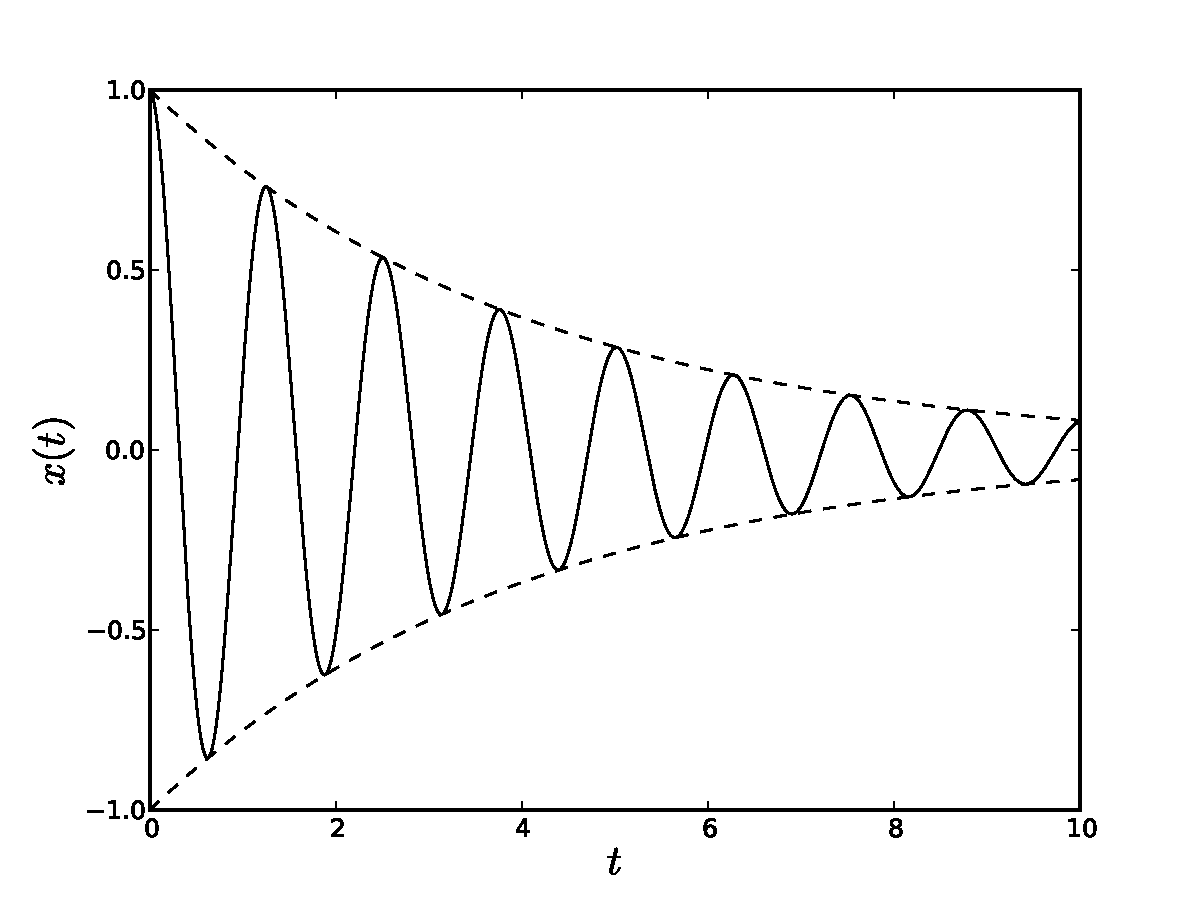
\includegraphics[scale=0.5]{damping}
  \caption{Oscilador amortiguado con }
  \label{fig:damping}
\end{figure}

La frecuencia característica ya depende también de la propiedades del fluido y es, a partir de  la ec.\eqref{eq:newoc}
\begin{align*}
  \omega_0\to \omega=&\sqrt{\omega_0^2-\frac{\gamma^2}{4}}\nonumber\\
=&\omega_0\sqrt{1-\left(\frac{1}{2}\frac{\gamma}{\omega}\right)^2}\,.
\end{align*}
Definimos el caso de amortiguamiento suave, la situación en la cual
\begin{align}
  \label{eq:SoftDamping}
  \frac{\gamma}{\omega}\ll 1\,,
\end{align}
tal que $\omega_0\approx\omega$. 

%definir los casos de poco, crittico y sobreamortiguado

El sistema ya no es conservativo de manera que la energía mecánica debe ser dependiente del tiempo

%  a un tiempo final $t$
% \begin{align}
%   \label{eq:Eoscamo}
%   E(t)-E(0)=W_{\text{fricc}}\,,
% \end{align}
% donde $W_{\text{fricc}}$ es la energía disipada por la fuerza de fricción
% \begin{align*}
%   W=&\int \mathbf{f}\cdot d \mathbf{r}\nonumber\\
%   =&\int \mathbf{f}\cdot \frac{d \mathbf{r}}{dt}\,dt\nonumber\\
%   =&\int \mathbf{f}\cdot  \mathbf{v}\,dt\nonumber\\
%   =&\int_0^t |\mathbf{f}| |\mathbf{v}|\cos(\pi)\,dt\nonumber\\
%   =&-b\int_0^tv^2(t) \,dt<0\,.
% \end{align*}
% de modo que la energía decrece con el tiempo. Para calcular $E(t)$,
\begin{align*}
  E(t)=&K(t)+U(t)\nonumber\\
=&\tfrac{1}{2}m v^2+\tfrac{1}{2}k x^2\,.
\end{align*}

Necesitamos $v(t)$. De \eqref{eq:soluflui}
\begin{align*}
  v=&\dot{x}=A_0 \left[-\frac{\gamma}{2}e^{-(\gamma/2)t}\cos(\omega t+\phi)+
            -\omega e^{-(\gamma/2)t}\sin(\omega t+\phi)\right]\nonumber\\
=&-A_0 \omega e^{-(\gamma/2)t} \left[\sin(\omega t+\phi)+\frac{1}{2}\frac{\gamma}{\omega}\cos(\omega t+\phi)\right].
\end{align*}

Aplicando la condición de amortiguamiento suave \eqref{eq:SoftDamping}
\begin{align*}
v\approx  -A_0 \omega e^{-(\gamma/2)t} \sin(\omega t+\phi),
\end{align*}
y reemplazando en la ecuación para la energía 
\begin{align*}
  E(t)\approx&\tfrac{1}{2}A_0^2 e^{-\gamma t} \left[
m\omega^2 \sin^2(\omega t+\phi)+k\cos^2(\omega t+\phi)\right]
\end{align*}
como en el límite de amortiguamiento suave $\omega_0\approx \omega$, $k=m\omega_0^2\approx m\omega^2$, y
\begin{align*}
  E(t)\approx&\tfrac{1}{2}k A_0^2 e^{-\gamma t} \left[
 \sin^2(\omega t+\phi)+\cos^2(\omega t+\phi)\right]\nonumber\\
=&\tfrac{1}{2}k A_0^2 e^{-\gamma t}\,.
\end{align*}
En $t=0$,
\begin{align*}
 E_0\equiv E(0)=\tfrac{1}{2}k A_0^2 \,,
\end{align*}
de modo que
\begin{align*}
  E(t)\approx E_0 e^{-\gamma t}\,.
\end{align*}
De modo que la energía mecánica decrece exponencialmente con el tiempo.  El decaimiento puede se caracterizado por el tiempo $\tau$ requerido para que la energía decaiga a $e^{-1}=0.368$ de su valor inicial %como se muestra en el plot
\begin{align*}
  E(\tau)=E_0 e^{-\gamma \tau}=E_0 e^{-1}\,.
\end{align*}
La condición para $\tau$ es entonces que
\begin{align*}
  \gamma \tau=&1\,,
\end{align*}
y
\begin{align}
  \label{eq:vidamedia}
  \tau=\frac{1}{\gamma}=\frac{m}{b}\,.
\end{align}
$\tau$ es el tiempo de amortiguamiento del sistema. Definimos el \emph{grado de amortiguamiento} como
\begin{align*}
  Q=\frac{\text{energía almacenada en el oscilador}}{\text{energía disipada por radian}}
\end{align*}

Energía perdida durante el tiempo que le toma al sistema oscilar por un radian.  En el tiempo $T$ el sistema oscila $2\pi$ radianes:
\begin{align*}
  T=\frac{2\pi\ \text{rad}}{\omega}
\end{align*}
El tiempo para oscilar por un radián es
\begin{align*}
  \Delta t\approx \frac{T}{2\pi}=\frac{2\pi/\omega}{2\pi}=\frac{1}{\omega}\,.
\end{align*}

Para el caso de amortiguamiento suave
\begin{align*}
  \frac{dE}{dt}=-\gamma E_0 e^{-\gamma t}=-\gamma E\,,
\end{align*}

La energía disipada en un intervalo de tiempo corto $\Delta t$ es la cantidad positiva
\begin{align*}
  \Delta E\approx\left|\frac{d E}{d t}\right|\Delta t=\gamma E \Delta t
\end{align*}
como un radian de oscilación toma un tiempo
\begin{align*}
  \Delta t=\frac{1}{\omega}\,,
\end{align*}
la energía disipada por radian es
\begin{align*}
  \gamma E \Delta t=\frac{\gamma}{\omega}\,,
\end{align*}
entonces
\begin{align}
  \label{eq:calidad}
  Q=\frac{E}{\gamma E \Delta t}=\frac{E}{\gamma E/\omega}=\frac{\omega}{\gamma}\,.
\end{align}
Un oscilador suavemente amortiguado satisface que $\omega\approx\omega_0$ y tiene
\begin{align*}
 Q \approx \frac{\omega_0}{\gamma}\gg 1\,.
\end{align*}
Es decir, un oscilador suavemente amortiguado tiene $Q\gg 1$. Un oscilador altamente amortiguado tiene un $Q$ bajo

\begin{itemize}
\item[\textbf{Ejemplo:}] \textbf{Gas de hidrógeno}. 
\end{itemize}

\subsection{Oscilador forzado y amortiguado}
Retornando a la solución general~\eqref{eq:soluforzamo} podemos estudiar como se comporta la amplitud en función de $\omega$. Los puntos extremos de la amplitud se encuentra derivando con respecto a $\omega$
\begin{align*}
\frac{d A(\omega)}{d\omega}=
  -\frac{(\mathcal{F}_0/m) \omega  \left(\gamma^2+2 \omega^2-2 \omega_0^2\right)}{
  \left[\left(\omega_0^2-\omega^2\right)^2+\gamma^2\omega^2\right]^{3/2}}
\end{align*}
La derivada es cero cuando
\begin{align*}
  \gamma^2+2 \omega^2-2 \omega_0^2=0
\end{align*}
y teniendo en cuenta que por definición $\omega$ es positiva, llegamos al punto extremo
\begin{align*}
  \tilde\omega=&\sqrt{\omega _0^2-\frac{\gamma^2}{2}}\nonumber\\
=&\omega_0\sqrt{1-\frac{1}{2}\frac{\gamma^2}{\omega_0^2}}\,.
\end{align*}
que está definido si
\begin{align}
  \label{eq:solcon}
  1-\frac{1}{2}\frac{\gamma^2}{\omega_0^2}>0\,.
\end{align}

La segunda derivada
\begin{align*}
  \frac{d^2A(\omega)}{d\omega}=
\frac{(\mathcal{F}_0/m) \left(2 \gamma ^4 \omega
   ^2+5 \gamma ^2 \omega ^4+\omega
   _0^4 \left(2 \omega ^2-\gamma
   ^2\right)-2 \omega _0^2 \left(4
   \gamma ^2 \omega ^2+5 \omega
   ^4\right)+6 \omega ^6+2 \omega
   _0^6\right)}{%
\left[\left(\omega_0^2-\omega^2\right)^2+\gamma^2\omega^2\right]^{5/2}}
\end{align*}
evaluada en el punto extremo $\tilde\omega$
\begin{align*}
  \left.\frac{d^2A(\omega)}{d\omega}\right|_{\omega=\tilde\omega}=&
  \frac{16 (\mathcal{F}_0/m) \left(\gamma^2-2 \omega_0^2\right) \sqrt{4 \gamma^2\omega_0^2-\gamma^4}}{
  \gamma^4 \left(\gamma^2-4 \omega_0^2\right)^2}\nonumber\\
=&
  -2\omega_0\left(1-\frac{1}{2}\frac{\gamma^2}{\omega_0^2}\right)\frac{16 (\mathcal{F}_0/m)  \sqrt{4 \gamma^2\omega_0^2-\gamma^4}}{\gamma^4 \left(\gamma^2-4 \omega_0^2\right)^2}\,.
\end{align*}
Como el primer término entre paréntesis es positivo de acuerdo a la ec.~\eqref{eq:solcon}, la segunda derivada es negativa, de manera que el punto $\tilde\omega$ en el gráfico de $A(\omega)$ en función de $\omega$ es un máximo. Al valor máximo de la amplitud $A(\tilde\omega)$ se le llama \emph{amplitud de resonancia} y a diferencia del caso sin amortiguamiento es finito.

Además
\begin{align}
  \lim_{\omega\to \pm\infty}A(\omega)=&
\lim_{\omega\to \pm\infty}\frac{\mathcal{F}_0}{m}\frac{1}{\left[\left(\omega_0^2-\omega^2\right)^2+\gamma^2\omega^2\right]^{1/2}}\nonumber\\
=&
\lim_{\omega\to \pm\infty}\frac{\mathcal{F}_0}{m}\frac{1}{\left[\omega^4\left(1-\frac{\omega_0^2}{\omega^2}\right)^2+\gamma^2\omega^2\right]^{1/2}}\nonumber\\
=&
\lim_{\omega\to \pm\infty}\frac{1}{\omega^2}\frac{\mathcal{F}_0}{m}\frac{1}{\left[\left(1-\frac{\omega_0^2}{\omega^2}\right)^2+\frac{\omega^2}{\gamma^2}\right]^{1/2}}\nonumber\\
=&0\,
\end{align}
%El gráfico generico se muestra en la figura

En el caso de amortiguamiento ligero correspondiente a
\begin{align*}
  \frac{\gamma}{\omega_0}\ll 1\,,
\end{align*}
El máximo valor de la amplitud se alcanza para $\omega=\tilde\omega=\omega_0$, y de la ec.~\eqref{eq:aomega}, tenemos que la amplitud en la resonancia es
\begin{align*}
  A(\omega_0)\approx&\frac{\mathcal{F}_0}{m\gamma\omega}\nonumber\\
\approx&\frac{\mathcal{F}_0}{m\gamma\omega_0}\,.
\end{align*}
A medida que $\gamma\to0$, $A(\omega_0)\to\infty$ como es de esperarse para un oscilador no amortiguado.


Para analizar la energía del sistema conveniente calcular la energía mecánica promedio del sistema, la cual será una función de la frecuencia impulsora. Como
\begin{align*}
  x=& A(\omega)\cos(\omega t +\phi)\nonumber\\
  v=& -A(\omega)\omega\sin(\omega t +\phi)\,.
\end{align*}
Entonces
\begin{align*}
  E(t)=\tfrac{1}{2}A^2(\omega)\left[m\omega^2\sin^2(\omega t+\phi)+k\cos^2(\omega t +\phi)\right]\,,
\end{align*}
mientras que la energía promedio sobre un período de la oscilación es
\begin{align*}
  \langle E(t)\rangle=&\tfrac{1}{4}A^2(\omega)(m\omega^2+k)\nonumber\\
=&\tfrac{1}{4}A^2(\omega)(m\omega^2+m\omega_0^2)\nonumber\\
=&\tfrac{1}{4}m A^2(\omega)(\omega^2+\omega_0^2)\nonumber\\
=&\frac{1}{4}\frac{\mathcal{F}_0^2}{m}\frac{(\omega^2+\omega_0^2)}{\left(\omega_0^2-\omega^2\right)^2+\gamma^2\omega^2}\nonumber\\
=&\frac{1}{4}\frac{\mathcal{F}_0^2}{m}\frac{\omega_0^2}{\omega_0^4}\frac{(1+{\omega^2}/{\omega_0^2})}{\left(1-\omega^2/\omega_0^2\right)^2+\gamma^2\omega^2/\omega_0^4}\nonumber\\
=&\frac{1}{4}\frac{\mathcal{F}_0^2}{m\omega_0^2}\frac{(1+{\omega^2}/{\omega_0^2})}{\left(1-\omega^2/\omega_0^2\right)^2+\gamma^2\omega^2/\omega_0^4}\,.
\end{align*}

Si $\omega\approx\omega_0$, en el límite de amortiguamiento suave $\gamma/\omega\ll1$
\begin{align*}
  \langle E(t)\rangle\approx&\frac{1}{4}\frac{\mathcal{F}_0^2}{m\omega_0^2}\frac{2}{(1-{\omega}/{\omega_0})^2(1+{\omega}/{\omega_0})^2+(\gamma^2/\omega_0^2)\omega^2/\omega_0^2}\nonumber\\
\approx&\frac{1}{4}\frac{\mathcal{F}_0^2}{m\omega_0^2}\frac{2}{(1-{\omega}/{\omega_0})^2(4)+(\gamma^2/\omega_0^2)}\nonumber\\
\approx&\frac{1}{8}\frac{\mathcal{F}_0^2}{m\omega_0^2}\frac{1}{(1-{\omega}/{\omega_0})^2+(\gamma^2/4\omega_0^2)}\nonumber\\
\approx&\frac{1}{8}\frac{\mathcal{F}_0^2}{m\omega_0^2}\frac{\omega_0^2}{(\omega_0-{\omega}/{\omega_0})^2+(\gamma/2)^2}\,,
\end{align*}
y
\begin{align*}
   \langle E(t)\rangle=&\frac{1}{8}\frac{\mathcal{F}_0^2}{m}
   \left[\frac{1}{(\omega-\omega_0)^2+(\gamma/2)^2}\right]\,,
\end{align*}
una función conocida como \emph{Lorentziana}.


Sí $\omega=\omega_0$, la parte
\begin{align*}
  h(\omega)\equiv\frac{1}{(\omega-\omega_0)^2+(\gamma/2)^2}\,,
\end{align*}
define la \emph{altura de la Lorentziana}
\begin{align*}
 h_0\equiv h(\omega_0)=\frac{1}{(\gamma/2)^2}=\frac{4}{\gamma^2}
\end{align*}
Además 
\begin{align*}
  \left.h(\omega)\right|_{(\omega-\omega_0)^2=(\gamma/2)^2}=\frac{h_0}{2}
\end{align*}
Definimos la \emph{amplitud de resonancia}, como la amplitud de la curva $\Gamma(\omega)$ en función de $\omega$ a la mitad del valor máximo. Dicha amplitud es la distancia en el eje $\omega$ entre un $\omega_+$ y $\omega_-$ que son solución a la ecuación
\begin{align*}
  (\omega-\omega_0)^2=(\gamma/2)^2\,,
\end{align*}
es decir,
\begin{align*}
  \omega_{\pm}=\pm \frac{\gamma}{2}\,.
\end{align*}
La amplitud de la resonancia es entonces
\begin{align*}
  \Delta\omega=\omega_+-\omega_-=\gamma
\end{align*}

A medida que $\gamma\to$ la curva se vuelve más alta y estrecha. De modo que el rango sobre el cual el sistema responde llega a ser más pequeño y el oscilador llega a ser cada vez más selectivo en frecuencia, de la ecuación para el factor de calidad \eqref{eq:calidad}, teníamos
\begin{align*}
Q=&\frac{\omega_0}{\gamma}\qquad\text{si}\ \frac{\gamma}{\omega}\ll 1  
\end{align*}
Como $\Delta\omega=\gamma$, entonces, el factor de calidad de  un oscilador forzado y suavemente amortiguado es
\begin{align*}
  Q=\frac{\omega_0}{\Delta \omega}=\frac{\text{frecuencia de resonancia}}{\text{amplitud de resonancia}}\,.
\end{align*}

$Q$ caracteriza la frecuencia de respuesta de un sistema, a medida que $Q$ crece, el sistema se vuelve más selectivo en frecuencias. Por ejemplo, en sistemas atómicos $Q\sim 10^8$ lo que implica que el sistema no genera ninguna respuesta a menos que sea forzado muy cerca a su amplitud de resonancia. Como la frecuencia de oscilación de dichos sistemas atómicos es independiente de influencias externas, la característica de tener alto $Q$ puede usarse en algunas aplicaciones como lo relojes atómicos. 

Note que entre más pequeño sea el amortiguamiento, menos energía se disipa. El tiempo de disipación de amortiguamiento del sistema  fue definido en la ec.~\eqref{eq:vidamedia}. En el caso de un oscilador forzado y suavemente amortiguado, dicho tiempo satisface la condición
\begin{align*}
  \tau \Delta \omega =1\,,
\end{align*}
que límite el diseño de osciladores. Si un elemento es muy selectivo en frecuencia entonces necesariamente oscila durante mucho tiempo. Además,  un elemento de estas característica le tomará mucho tiempo regresar al reposo después de aplicar una fuerza impulsora adecuada. 

En mecánica cuántica existe una relación similar que corresponde al \emph{principio de incertidumbre}
\begin{align*}
  \Delta t \Delta E\ge \frac{\hbar}{2}
\end{align*}
que limita la respuesta de los sistemas cuánticos. 

\begin{itemize}
\item[\textbf{Ejemplo:}] La partícula $Z$ corresponde a una resonancia centrada en $91.1876\pm 0.0021$~GeV y con una amplitud de $2.4952\pm0.023$\~GeV (En unidades naturales). ¿cual es el tiempo de amortiguamiento (en este caso de decaimiento) de la resonanciaP?, ¿Cual es el factor de Calidad? 

\item[\textbf{Solución}]. El factor de conversión de GeV  a segundos es
  \begin{align*}
    1\ \text{GeV}^{-1}=6.58211899\times 10^{-25}\second\,,
  \end{align*}
  Entonces
  \begin{align*}
    \tau=\frac{1}{\gamma}=2.6379\times10^{-25}\second\,.
  \end{align*}
  \begin{align*}
    Q=\frac{\omega_0}{\gamma}=36.5
  \end{align*}
\end{itemize}
%ejemplos

%\left(\right)

%%% Local Variables: 
%%% mode: latex
%%% TeX-master: "mecanica"
%%% End: 
